\section{Arrays and talloc}
\label{talloc:sec:arrays}

The following sections describe the array interface and special properties that
talloc implements. Namely how to create, manage and free an array and how to
determine its length from the context size.

\subsection{Creating a new array}

We are already able to create an array with the knowledge introduced in the
previous text. We can do it in the same way as in the C standard library using
|talloc_size()| where the size of the context would be |sizeof(type) *|
|number_of_elements|.

However, this has two disadvantages. First of all we have to use the type unsafe
functions to allocate the requested size which is unreliable. And at second,
we have to do the multiplication by ourselves. Talloc developers were aware of
it and they have created a separate interface for arrays:

\begin{funcproto}
(#type)* talloc_array(TALLOC_CTX *ctx, #type,
                      unsigned int count)
(#type)* talloc_zero_array(TALLOC_CTX *ctx, #type
                           unsigned int count)
void* talloc_array_size(TALLOC_CTX *ctx, size_t size,
                        unsigned int count)
void* talloc_array_ptrtype(TALLOC_CTX *ctx, #ptrtype,
                           unsigned int count)
\end{funcproto}
\funclistend
Or to reallocate the array use:

\begin{funcproto}
void* talloc_realloc(TALLOC_CTX *parent,
                     TALLOC_CTX *ctx,
                     #type, size_t count)
void* talloc_realloc_size(TALLOC_CTX *parent,
                          TALLOC_CTX *ctx,
                          size_t size)
\end{funcproto}
\begin{funcdesc}
If |ctx| is |NULL| a new context is created. If |count| or |size| is zero, it
will free the context. The memory occupied by |ctx| may be moved to other
location, therefore always replace it by the returned pointer.
\end{funcdesc}
\funclistend
We should always project the natural structure of an array into talloc context
hierarchy. That is, the array should be always used as a parent of its
dynamically created elements.

\begin{lstlisting}[caption={Array of users and context hierarchy},
label={array-users}] int i, j;
struct user **users;
users = talloc_zero_array(NULL, struct user*, N + 1);

for (i = 0; i < N; i++) {
  users[i] = talloc_zero(users, struct user);
  users[i]->num_groups = i;
  users[i]->groups = talloc_zero_array(users[i], char*, i);
  
  for (j = 0; j < i; j++) {
    users[i]->groups[j] = talloc_asprintf(
                          users[i]->groups[j],"Group %d",j);
  }
}
\end{lstlisting}

This way we gain a lot of flexibility. We do not have to free every element
separately to deallocate the whole array, we can achieve this simply by calling
|talloc_free(users)|. Or we can move any part of the array to another parent
context to keep it accessible even if we free the array later.

The context tree that graphically illustrates the hierarchy from previous
listing can be find on Figure \ref{fig:context-tree-array}.

\begin{figure}[H]
  \centering
  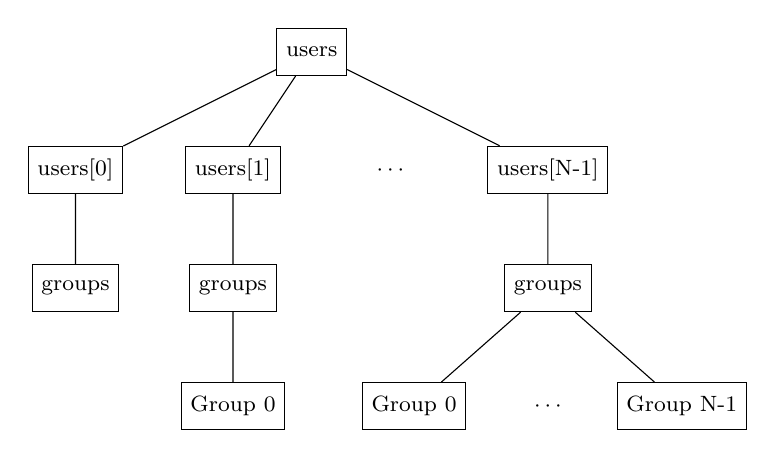
\begin{tikzpicture}
[level/.style={sibling distance=17mm},
 level 1/.style={sibling distance=20mm},
 every node/.style=
   {minimum height=6mm,rectangle,draw=black,font=\footnotesize}]
\node [] {users}
  child {node [] {users[0]}
    child {node [] {groups}
    }
  }
  child {node [] {users[1]} 
    child {node [] {groups}
      child {node [] {Group 0} }
    }
  }
  child {node [draw=none] {$\cdots$} edge from parent[draw=none]}
  child {node [] {users[N-1]}
    child {node [] {groups}
      child {node [] {Group 0} }
      child {node [draw=none] {$\cdots$} edge from parent[draw=none]}
      child {node [] {Group N-1} }
    }
  };
\end{tikzpicture}
  \caption{Context tree from Listing \ref{array-users}}
  \label{fig:context-tree-array}
\end{figure}

\subsection{Determining the length of an array}

We can find ourselves in a situation when we need to iterate through an array
but we are not able or we do not want to use a special delimiter to mark the
end of the array. We need to store the size of the array in other variable and
carry this information with the array.

Talloc makes this easier as every talloc context already contains the
information about its size (in bytes). Therefore, instead of carrying the number
of the elements separately, we can just divide the context size by the size of
the data type the array consists of. Talloc has a macro
|talloc_array_length(ctx)| that serves for this purpose. It requires the name of
the context to be the name of the data type. Thus if we want to use this
feature, we should use the type safe functions to create the array.

\begin{lstlisting}[caption={Length of an array},label=lst:array-length]
TALLOC_CTX *ctx = talloc_new(NULL);
int *i = talloc_zero(ctx, int);
char *str = talloc_strdup(ctx, "hello world");
int *array = talloc_array(ctx, int, 10);

printf("%lu\n", talloc_array_length(ctx));   /*  0 */
printf("%lu\n", talloc_array_length(i));     /*  1 */
printf("%lu\n", talloc_array_length(str));   /* 12 */
printf("%lu\n", talloc_array_length(array)); /* 10 */

talloc_free(ctx);
\end{lstlisting}

It can be also used as a more efficient way of computing a number of characters
in a string that has been created with talloc library. However, we need to
create our own function (or macro) to do this. Although we must be very careful
with the usage as it will misbehave once we put a |'\0'| character inside the
string, having that on mind we will gain the constant complexity. For example:

\begin{lstlisting}[caption={Length of a string},label=lst:array-length]
size_t talloc_strlen(const char *str)
{
  return talloc_array_length(ctx) - 1;
}

char *str = talloc_strdup(ctx, "hello world");
char *str2 = talloc_strdup(ctx, "hello world");
str2[5] = '\0';

printf("%lu\n", talloc_strlen(str));   /* 11 */
printf("%lu\n", talloc_strlen(str2));  /* (*@{\ttfamily\bf 11}@*) */
printf("%lu\n", strlen(str2));         /* (*@{\ttfamily\bf 5 !}@*) */
\end{lstlisting}